\documentclass[11pt]{article}
\usepackage[margin=0cm,nohead]{geometry}
\usepackage[active,tightpage]{preview}

\usepackage{tikz,amsmath,amssymb,mathtools,mathrsfs,bm,color,cancel}

%\usepackage{newtxtext}
%\usepackage{newtxmath}

\usetikzlibrary{shapes,arrows}
\usetikzlibrary{calc}
\usetikzlibrary{positioning}
\usetikzlibrary{decorations.pathreplacing}
\usetikzlibrary{decorations.markings}
\usetikzlibrary{decorations.pathmorphing}

\PreviewEnvironment{tikzpicture}
\setlength\PreviewBorder{-1mm}

\begin{document}

\begin{tikzpicture}

%%%%%%%%%%%%%%%%%%%%%%%%%%%%%%%%%%%%%%%%%%%%%%%%%%%%%%%%%%%%%% Macros

\newcommand{\bb}[2]{
	\!\!{\tt #1}
	\\[6pt]
	~{\large \color{blue} #2}
}
\newcommand{\bbb}[3]{
	\!\!{\tt #1}
	\\[6pt]
	~{\large \color{blue} #2}
	\\[6pt]
	~{#3}
}

\newcommand{\textsfb}[1]{\textsf{{\textbf{#1}}}}

\newcommand{\tr}{\mathsf{{\scriptscriptstyle T}}}
\newcommand{\ii}{\mathrm{i}}
\newcommand{\ee}{\operatorname{e}}
\newcommand{\dd}{\mathrm{d}}
\newcommand{\op}[1]{\operatorname{#1}}

\newcommand{\pL}{\mathsf{{\scriptscriptstyle L}}}
\newcommand{\pR}{\mathsf{{\scriptscriptstyle R}}}
\newcommand{\pC}{\mathsf{{\scriptscriptstyle C}}}

\newcommand{\bPsi}{\boldsymbol{\Psi}}
\newcommand{\bPhi}{\boldsymbol{\Phi}}

\newcommand{\suY}{\mathrm{\scriptscriptstyle Y}}
\newcommand{\suL}{\mathrm{\scriptscriptstyle L}}
\newcommand{\suC}{\mathrm{\scriptscriptstyle C}}

\newcommand{\dbar}[1]{\overline{#1}}
\newcommand{\sbar}[1]{\bar{#1}}
\newcommand{\anti}[1]{\bar{#1}}

\newcommand{\eH}{\mathrm{\scriptscriptstyle H}}
\newcommand{\eC}{\mathrm{\scriptscriptstyle C}}

\newcommand{\quantNo}[3]{\mathbf{#1},\mathbf{#2},#3}

\newcommand{\midarrow}{\tikz \draw[-triangle 45] (0,0) -- +(0,0.1);}
\newcommand{\midarroww}{\tikz \draw[-triangle 45] (0,0) -- +(0,-0.1);}
\newcommand{\midarrowh}{\tikz \draw[-triangle 45] (0,0) -- +(0.1,0);}
\newcommand{\midarrowhh}{\tikz \draw[-triangle 45] (0,0) -- +(-0.1,0);}

\newcommand{\coSys}[1]{
	\node [left = 3.6mm of #1] {$v$};
	\node [below = 4mm of #1] {$r$};
	\draw [-triangle 45,thick] (#1) +(-10mm,-10mm) -- +(-10mm,0);
	\draw [-triangle 45,thick] (#1) +(-10mm,-10mm) -- +(0,-10mm);
	%\fill (#1) +(-10mm,-10mm) circle [radius=0.5mm];
}

\newcommand{\coSysU}[1]{
	\node [left = 3.6mm of #1] {$u$};
	\node [below = 4mm of #1] {$r$};
	\draw [-triangle 45,thick] (#1) +(-10mm,-10mm) -- +(-10mm,0);
	\draw [-triangle 45,thick] (#1) +(-10mm,-10mm) -- +(0,-10mm);
	%\fill (#1) +(-10mm,-10mm) circle [radius=0.5mm];
}

%%%%%%%%%%%%%%%%%%%%%%%%%%%%%%%%%%%%%%%%%%%%%%%%%%%%%%%%%%%%%% Box styles

\tikzset{myRow/.style     ={draw,anchor=north west,rectangle}}
\tikzset{boxWhite/.style  ={draw,anchor=north west,rectangle, very thin, rounded corners=5pt, fill=white}}
\tikzset{boxGray/.style   ={draw,anchor=north west,rectangle, very thin, rounded corners=5pt, fill=gray!10}}
\tikzset{boxRed/.style    ={draw,anchor=north west,rectangle, very thin, rounded corners=5pt, fill=red!4}}
\tikzset{boxGreen/.style  ={draw,anchor=north west,rectangle, very thin, rounded corners=5pt, fill=green!2}}
\tikzset{boxYellow/.style ={draw,anchor=north west,rectangle, very thin, rounded corners=5pt, fill=yellow!5}}
\tikzset{boxBlue/.style   ={draw,anchor=north west,rectangle, very thin, rounded corners=5pt, fill=blue!2}}
\tikzset{boxCyan/.style   ={draw,anchor=north west,rectangle, very thin, rounded corners=5pt, fill=cyan!2}}
\tikzset{colorLagr/.style ={fill=magenta!8}}

%%%%%%%%%%%%%%%%%%%%%%%%%%%%%%%%%%%%%%%%%%%%%%%%%%%%%%%%%%%%%% Row/Column styles

\tikzset{R/.style={
	minimum height = #1 mm
}}

\tikzset{C/.style={
    minimum width = #1 mm, 
    text width = #1 mm - 3 mm,
    inner sep = 0
}}

%%%%%%%%%%%%%%%%%%%%%%%%%%%%%%%%%%%%%%%%%%%%%%%%%%%%%%%%%%%%%%%%%%%%%%%%%%%%%%%

\tikzset{
	pics/cone/.style = {
	  code = {
	    \draw [fill=yellow!80,join=round,opacity=0.5] (3,-3) -- (0,0) -- (3,3);
	    \draw [fill=yellow!15](3.1,0) ellipse (.6 and 3.05);
	  }
	}
}

\tikzset{
	pics/conee/.style = {
	  code = {
	    \draw [fill=yellow!80,join=round,opacity=0.5] (3,-7.1) -- (0,0) -- (3,7.1);
	    \draw [fill=yellow!15](3.1,0) ellipse (.6 and 7.25);
	  }
	}
}

%%%%%%%%%%%%%%%%%%%%%%%%%%%%%%%%%%%%%%%%%%%%%%%%%%%%%%%%%%%%%%%%%%%%%%%%%%%%%%%

\tikzset{cross/.style={
	cross out, thick, draw=black, inner sep=0pt, outer sep=0pt,
	minimum size=1.5mm}
};

%%%%%%%%%%%%%%%%%%%%%%%%%%%%%%%%%%%%%%%%%%%%%%%%%%%%%%%%%%%%%% Paper W/H

% \draw [blue!40] (-20.5,14.5) rectangle (20.5,-14.5);

\node at (-20.5,14.5) {}; \node at (20.5,-14) {};

%%%%%%%%%%%%%%%%%%%%%%%%%%%%%%%%%%%%%%%%%%%%%%%%%%%%%%%%%%%%%% Title

\node [color=black] at (0,14.25) {
	\huge\sf Null Radial Geodesics \& Penrose-Carter Diagrams, 
	The Catalogue
};

\node [anchor=north, color=black] at (0,13.9) {
	by M.B.Kocic ~--~ Version 1.01 (2017-02-16)
};

\pdfinfo {
	%/CreationDate	(D:20170216124500)
	/Title			(Null Radial Geodesics & Penrose-Carter Diagrams, The Catalogue)
	/Author			(Mikica B Kocic)
	/Subject		(FK8017 HT15)
	/Keywords		(Null Cone, Geodesic, Penrose-Carter Diagram)
	/Creator		(TeX-TikZ)
}

%%%%%%%%%%%%%%%%%%%%%%%%%%%%%%%%%%%%%%%%%%%%%%%%%%%%%%%%%%%%%%

\node [boxYellow,anchor=north west,R=15,C=60] at (-20.5,10.3) {
	\textsfb{Minkowski}\\[5pt]
	\qquad $ F = 1 $
};


\node [] at (16.5,5) {
	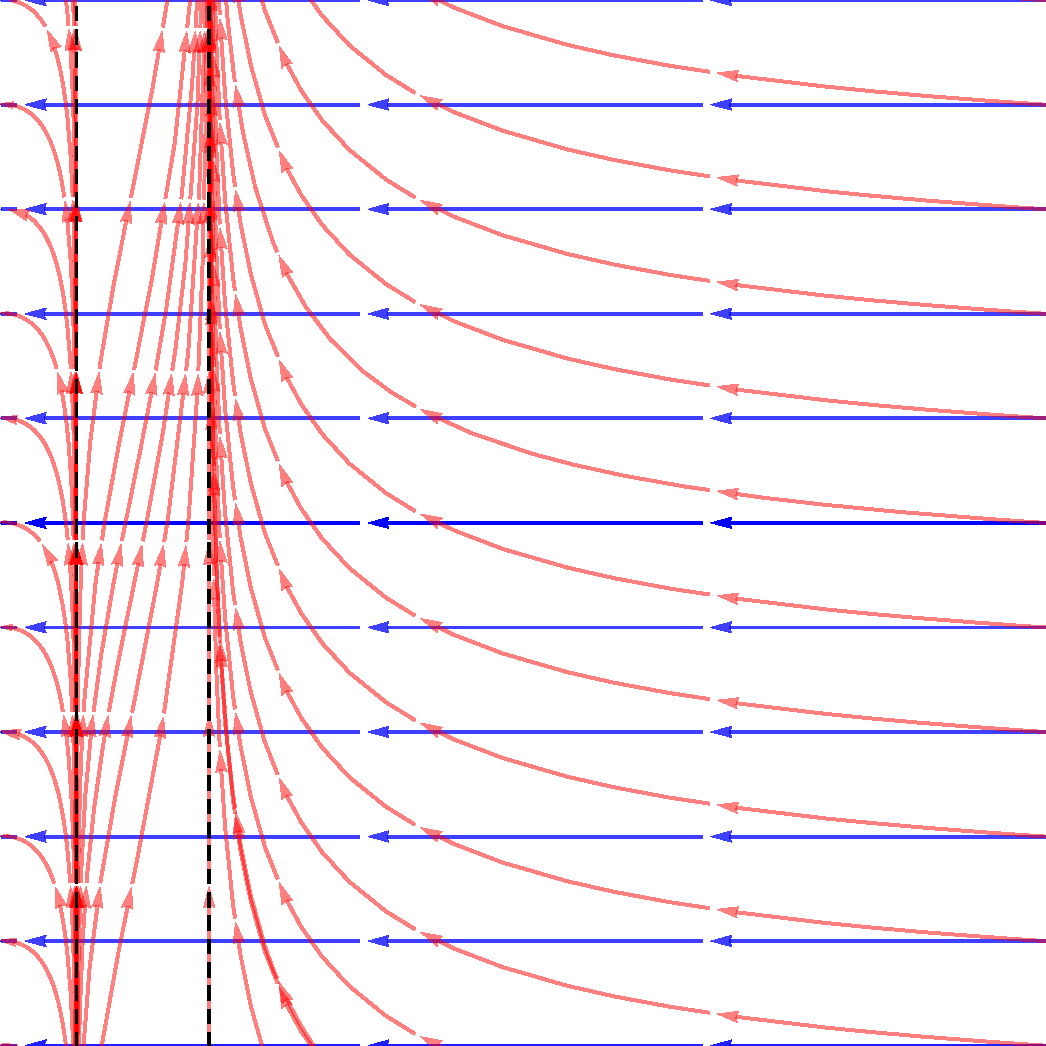
\includegraphics[width=80mm,height=60mm]{fig-S-dS-in.pdf}
};

\node [] at (16.5,-2.25) {
	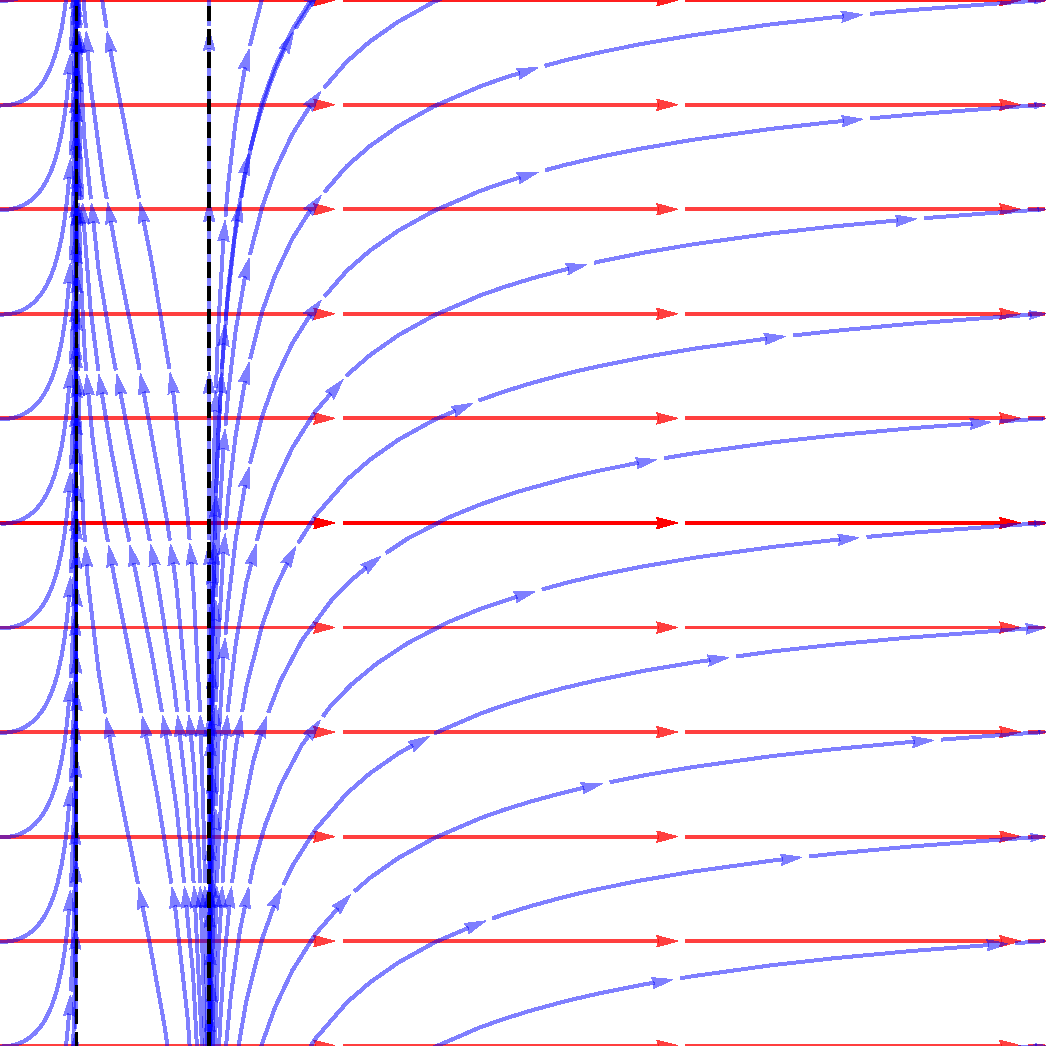
\includegraphics[width=80mm,height=60mm]{fig-S-dS-out.pdf}
};

%%%%%%%%%%%%%%%%%%%%%%%%%%%%%%%%%%%%%%%%%%%%%%%%%%%%%%%%%%%%%%

\node [boxYellow,anchor=north west,R=15,C=60] at (-1,10.3) {
	\textsfb{Schwarzschild}\\[3pt]
	\qquad $ F = 1 - \dfrac{r_\eH}{r}, 
	\quad r_\eH > 0$
};

\node [] at (2,5) {
	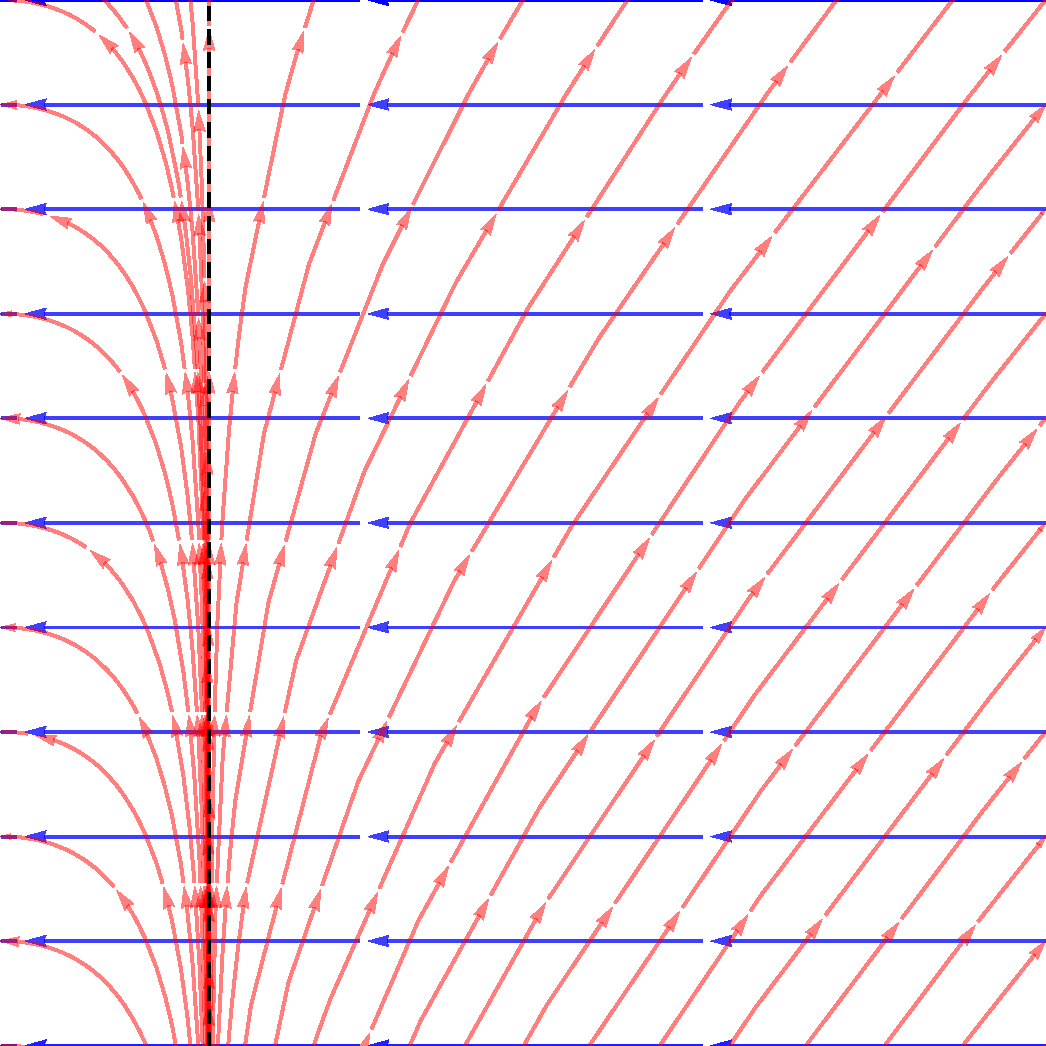
\includegraphics[width=60mm]{fig-Sch-in.pdf}
};

\node [] at (2,-2.25) {
	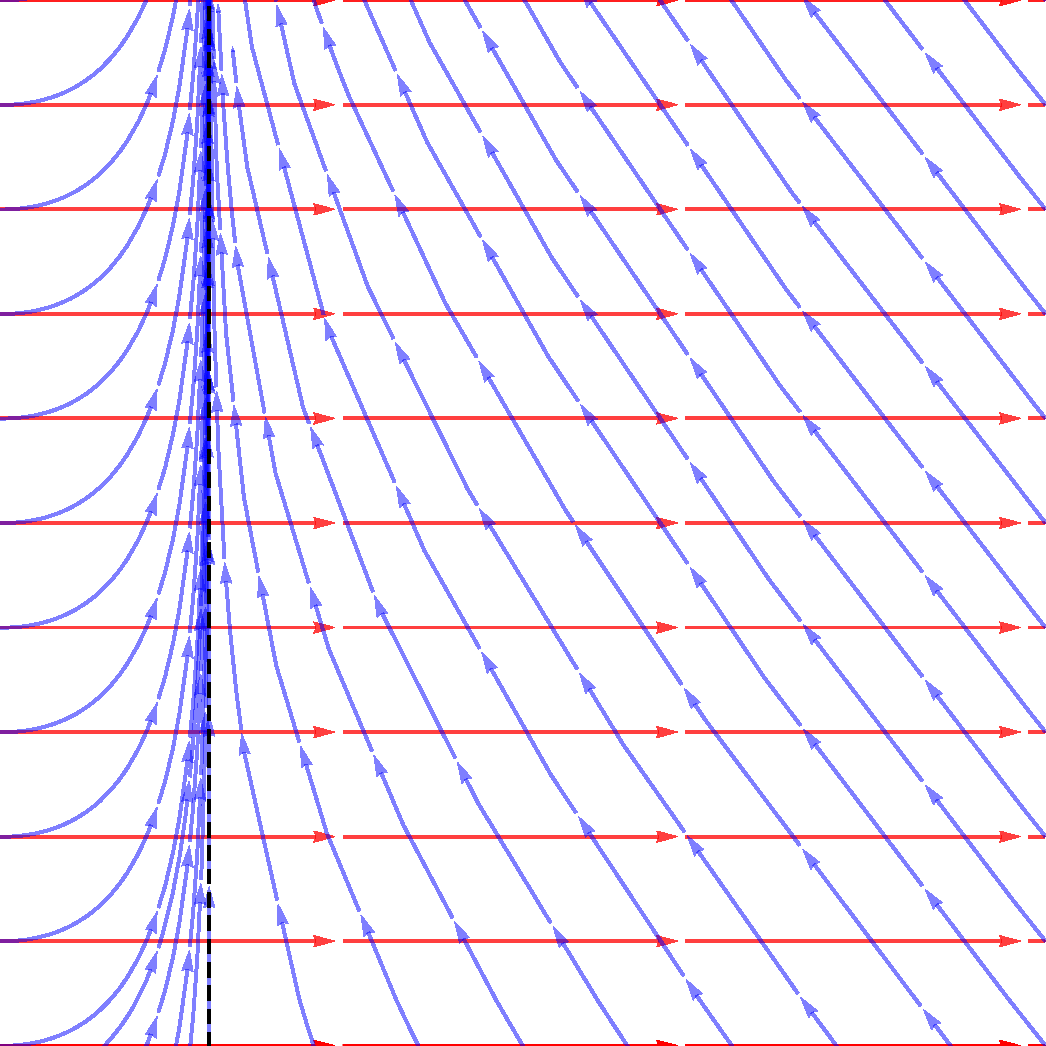
\includegraphics[width=60mm]{fig-Sch-out.pdf}
};

%%%%%%%%%%%%%%%%%%%%%%%%%%%%%%%%%%%%%%%%%%%%%%%%%%%%%%%%%%%%%%

\node [boxYellow,anchor=north west,R=15,C=60] at (5.5,10.3) {
	\textsf{Schwarzschild - Anti de Sitter}\\[2pt]
	\qquad $ F = 1 - \dfrac{r_\mathrm{\scriptscriptstyle S}}{r} - \dfrac{\Lambda}{3} r^2, 
	\quad \Lambda < 0 $
};

\node [] at (8.5,5) {
	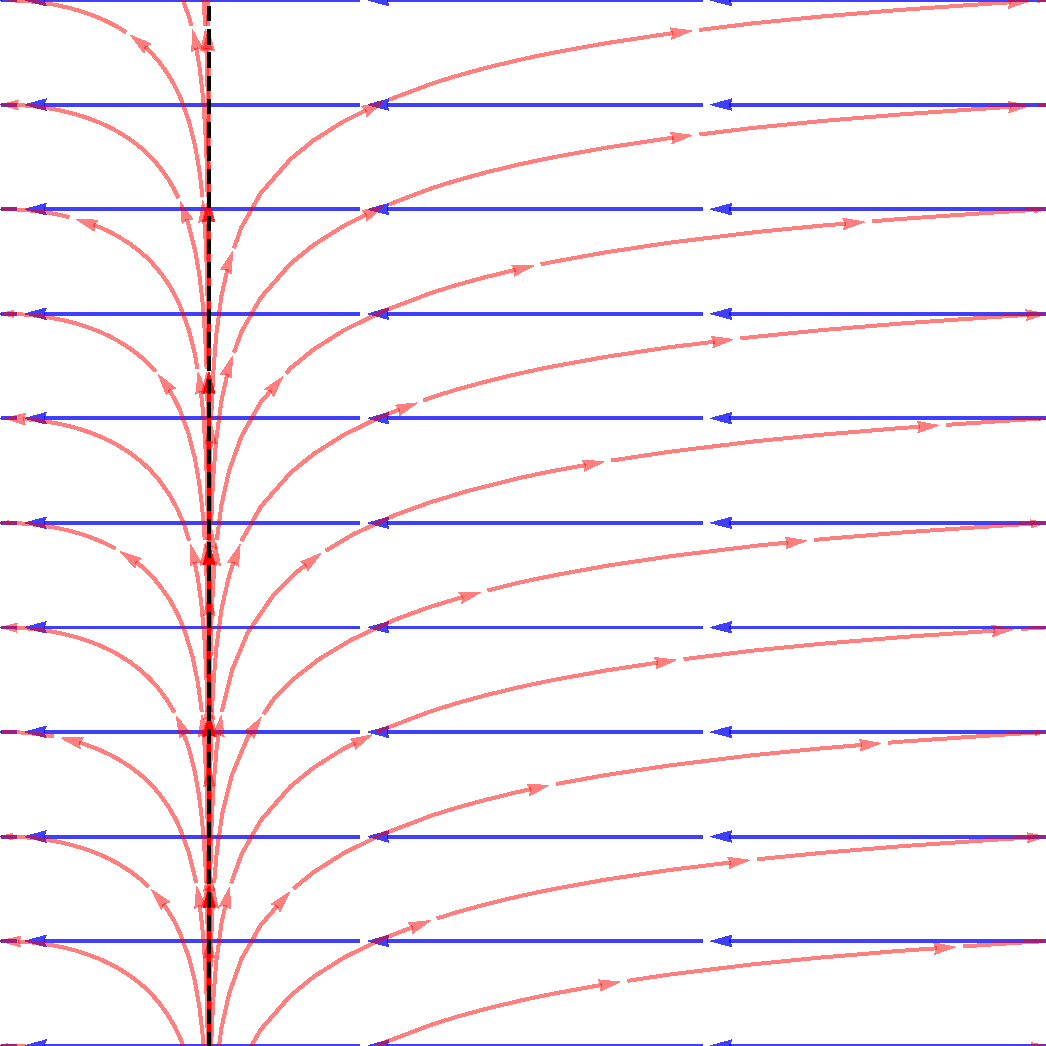
\includegraphics[width=60mm]{fig-S-AdS-in.pdf}
};

\node [] at (8.5,-2.25) {
	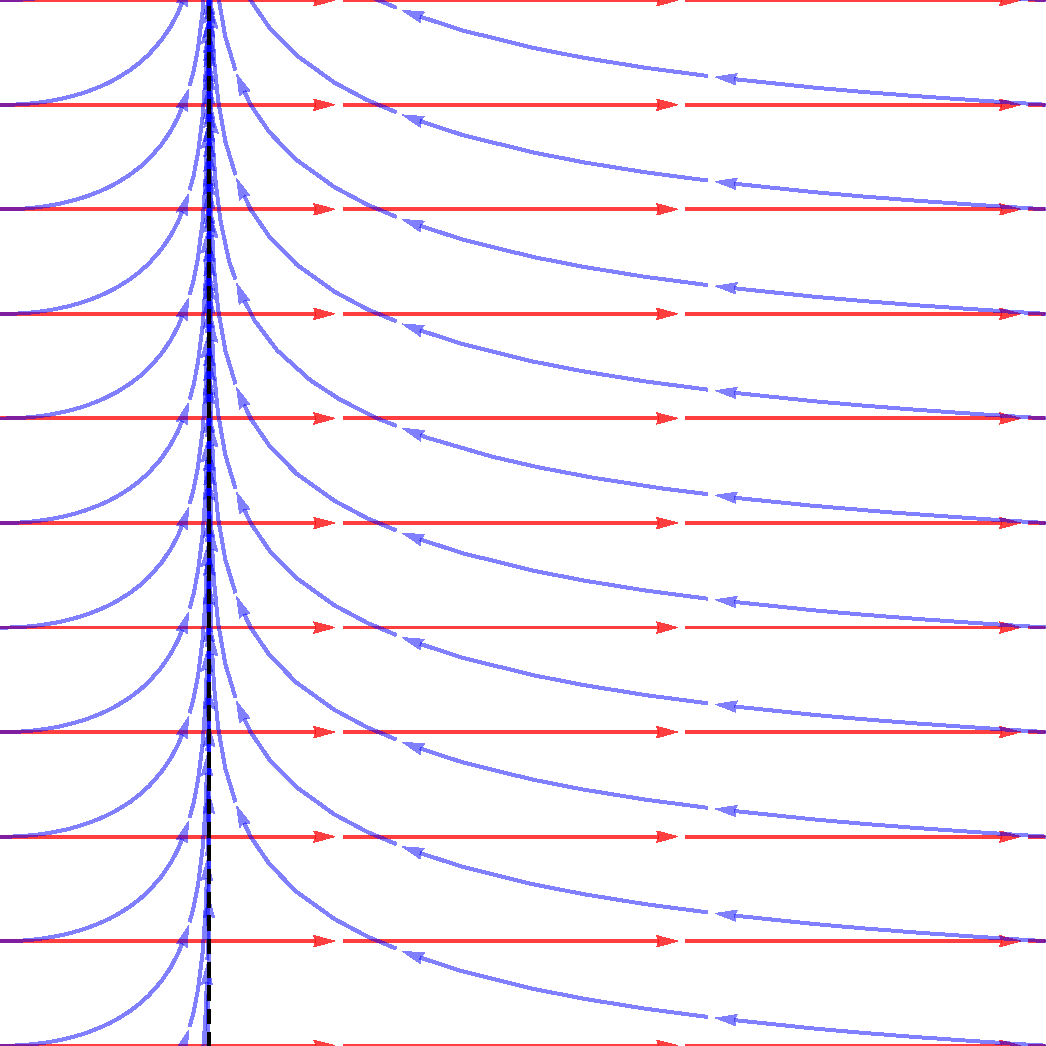
\includegraphics[width=60mm]{fig-S-AdS-out.pdf}
};

\node [fill=white] at (10,3) {
	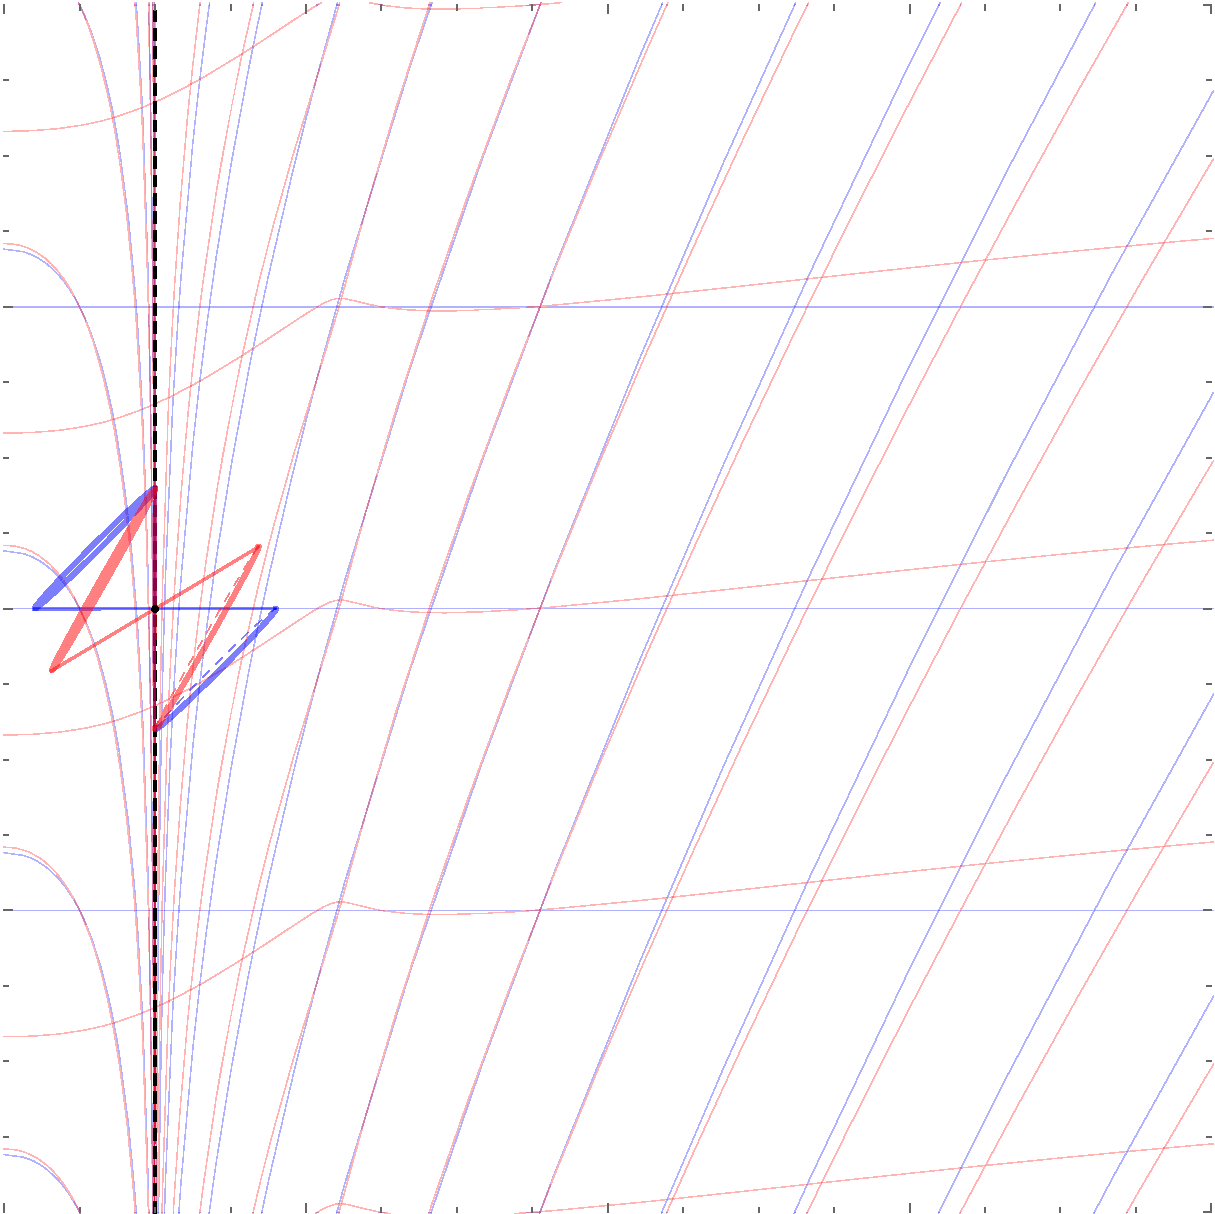
\includegraphics[width=30mm]{fig-Bim-S-AdS-in.pdf}
};

\node [] at (10.3,4.15) {Bim S-AdS};

%%%%%%%%%%%%%%%%%%%%%%%%%%%%%%%%%%%%%%%%%%%%%%%%%%%%%%%%%%%%%%

\node [boxYellow,anchor=north west,R=15,C=60] at (-14,10.3) {
	\textsf{Anti de Sitter}\\[2pt]
	\qquad $ F = 1 - \dfrac{\Lambda}{3} r^2, \quad \Lambda < 0 $
};

\node [] at (-17.5,5) {
	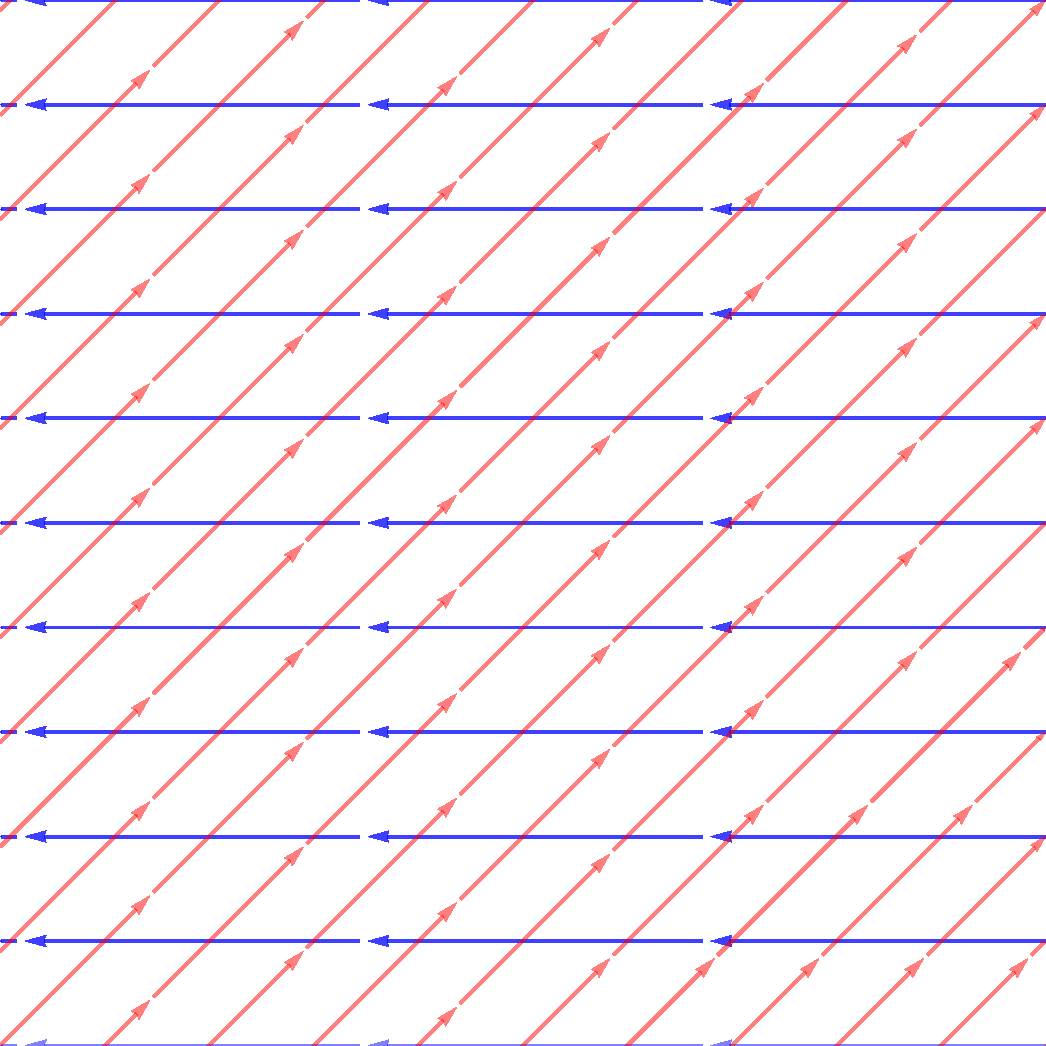
\includegraphics[width=60mm]{fig-Minkowski-in.pdf}
};

\node [] at (-17.5,-2.25) {
	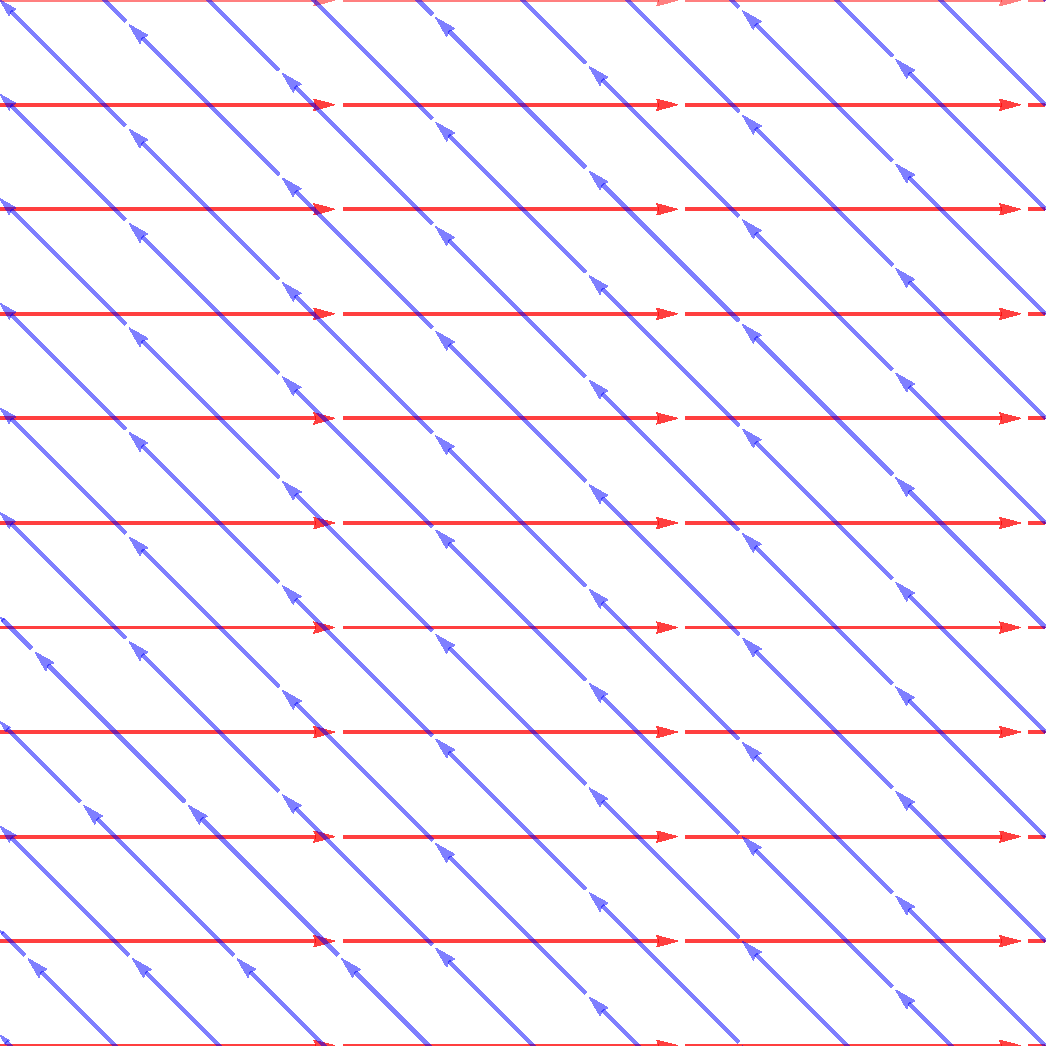
\includegraphics[width=60mm]{fig-Minkowski-out.pdf}
};

%%%%%%%%%%%%%%%%%%%%%%%%%%%%%%%%%%%%%%%%%%%%%%%%%%%%%%%%%%%%%%

\node [boxYellow,anchor=north west,R=15,C=60] at (-7.5,10.3) {
	\textsf{de Sitter}\\[2pt]
	\qquad $ F = 1 - \dfrac{\Lambda}{3} r^2,
	\quad \Lambda > 0 $
};

\node [] at (-11,5) {
	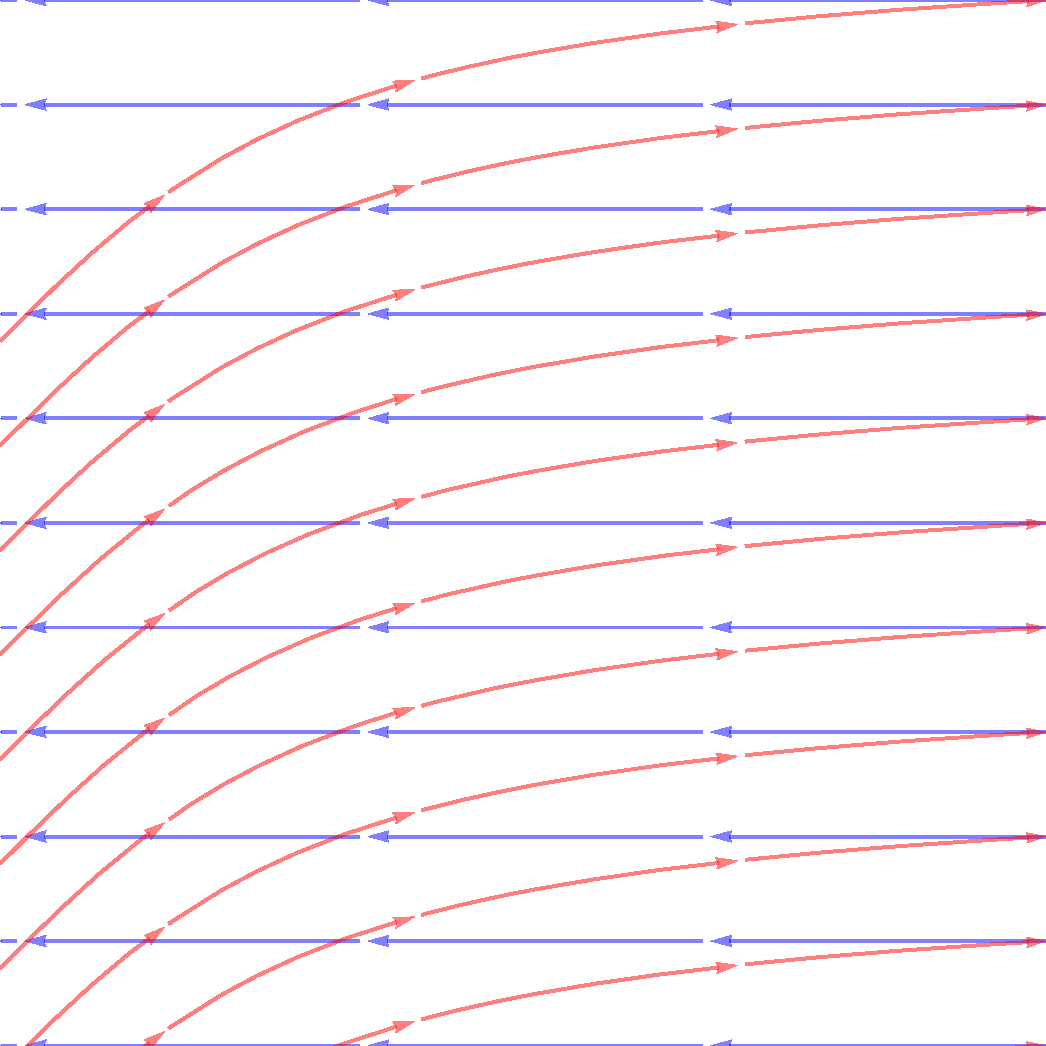
\includegraphics[width=60mm]{fig-AdS-in.pdf}
};

\node [] at (-11,-2.25) {
	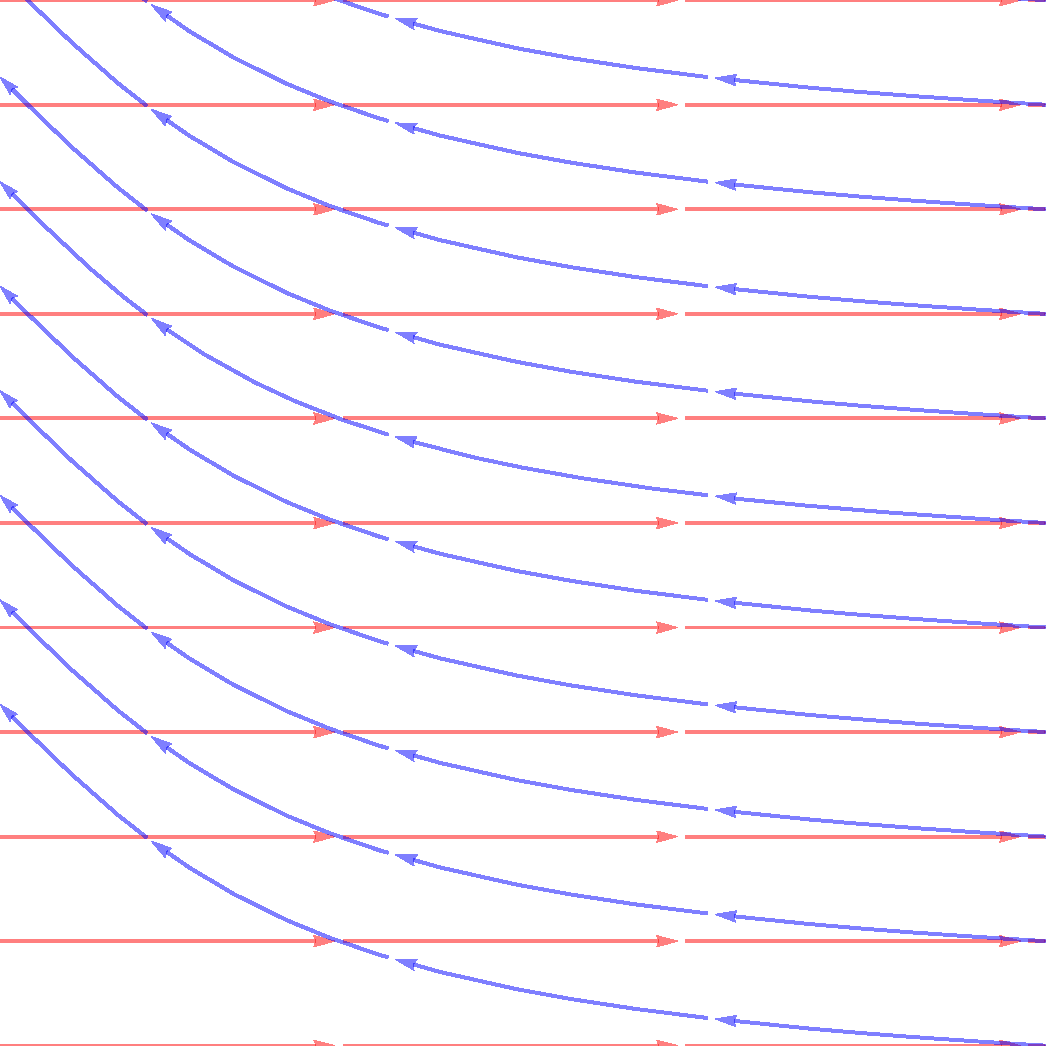
\includegraphics[width=60mm]{fig-AdS-out.pdf}
};

%%%%%%%%%%%%%%%%%%%%%%%%%%%%%%%%%%%%%%%%%%%%%%%%%%%%%%%%%%%%%%

\node [boxYellow,anchor=north west,R=15,C=80] at (12.5,10.3) {
	\textsf{Schwarzschild - de Sitter}\\[2pt]
	\qquad $ F = 1 - \dfrac{r_\mathrm{\scriptscriptstyle S}}{r} - \dfrac{\Lambda}{3} r^2,
	\quad \Lambda > 0 $
};

\node [] at (-4.5,5) {
	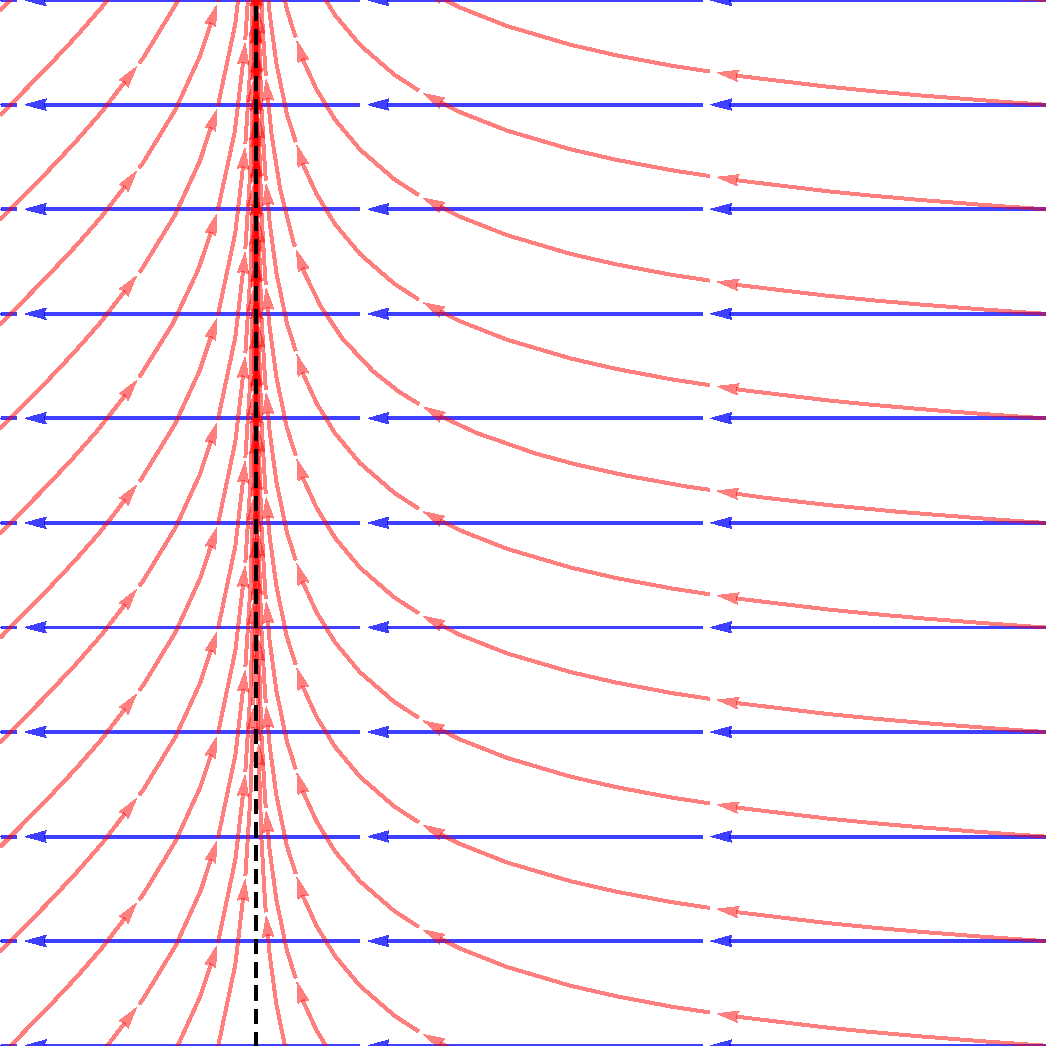
\includegraphics[width=60mm]{fig-dS-in.pdf}
};

\node [] at (-4.5,-2.25) {
	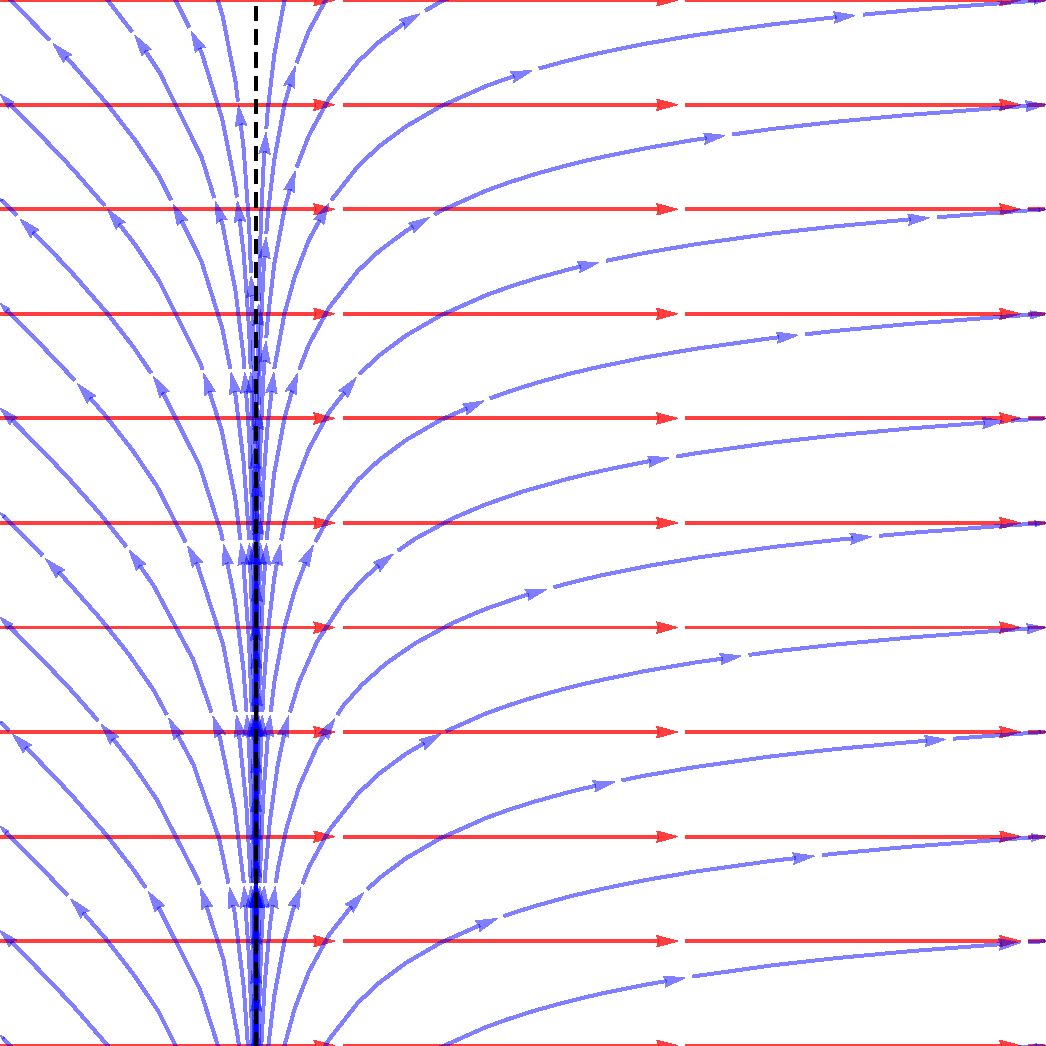
\includegraphics[width=60mm]{fig-dS-out.pdf}
};


%%%%%%%%%%%%%%%%%%%%%%%%%%%%%%%%%%%%%%%%%%%%%%%%%%%%%%%%%%%%%%

\draw [decorate,decoration={snake}](-1,2) -- (-1,7.5);
\draw [decorate,decoration={snake}](-1,-5.25) -- (-1,0.25);

\draw [decorate,decoration={snake}](5.5,2) -- (5.5,7.5);
\draw [decorate,decoration={snake}](5.5,-5.25) -- (5.5,0.25);

\draw [dotted](-20.5,3) -- (-20.5,7.5);
\draw [dotted](-20.5,-5.25) -- (-20.5,0.25);

\draw [dotted](-14,2) -- (-14,7.5);
\draw [dotted](-14,-5.25) -- (-14,0.25);

\draw [dotted](-7.5,2) -- (-7.5,7.5);
\draw [dotted](-7.5,-5.25) -- (-7.5,0.25);

\draw [decorate,decoration={snake}](12.5,2) -- (12.5,7.5);
\draw [decorate,decoration={snake}](12.5,-5.25) -- (12.5,0.25);

%%%%%%%%%%%%%%%%%%%%%%%%%%%%%%%%%%%%%%%%%%%%%%%%%%%%%%%%%%%%%%

\node [boxBlue,R=9,C=60] at (-20.5,8.25) {\textsf{Ingoing chart} $(v,r)$};
\node [boxBlue,R=9,C=60] at (-14,8.25) {\textsf{Ingoing chart} $(v,r)$};
\node [boxBlue,R=9,C=60] at (-7.5,8.25) {\textsf{Ingoing chart} $(v,r)$};
\node [boxBlue,R=9,C=80] at (12.5,8.25) {\textsf{Ingoing chart} $(v,r)$};
\node [boxBlue,R=9,C=60] at (-1,8.25) {\textsf{Ingoing chart} $(v,r)$};
\node [boxBlue,R=9,C=60] at (5.5,8.25) {\textsf{Ingoing chart} $(v,r)$};

\node [boxRed,R=9,C=60] at (-20.5,1) {\textsf{Outgoing chart} $(u,r)$};
\node [boxRed,R=9,C=60] at (-14,1) {\textsf{Outgoing chart} $(u,r)$};
\node [boxRed,R=9,C=60] at (-7.5,1) {\textsf{Outgoing chart} $(u,r)$};
\node [boxRed,R=9,C=80] at (12.5,1) {\textsf{Outgoing chart} $(u,r)$};
\node [boxRed,R=9,C=60] at (-1,1) {\textsf{Outgoing chart} $(u,r)$};
\node [boxRed,R=9,C=60] at (5.5,1) {\textsf{Outgoing chart} $(u,r)$};

\node at (-19.25,-7) {\textsfb{Minkowski}};
\node at (-13.25,-7) {\textsfb{de Sitter}};
\node at (-4,-7) {\textsfb{Schwarzschild}};
\node at (5,-7) {\textsfb{Schwarzschild - Anti de Sitter}};
\node at (14.5,-7) {\textsfb{Schwarzschild - de Sitter}};

%%%%%%%%%%%%%%%%%%%%%%%%%%%%%%%%%%%%%%%%%%%%%%%%%%%%%%%%%%%%%%

\node [anchor=north west,R=6] at (-20.75,2) {$r = 0$};
\node [anchor=north west,R=6] at (-14.25,2) {$r = 0$};
\node [anchor=north,R=6] at (-7.5,2) {$r = 0$};
\node [anchor=north,R=6] at (-1,2) {$r = 0$};
\node [anchor=north,R=6] at (5.5,2) {$r = 0$};
\node [anchor=north,R=6] at (12.5,2) {$r = 0$};

\node [anchor=north west,R=6] at (-20.75,-5.25) {$r = 0$};
\node [anchor=north west,R=6] at (-14.25,-5.25) {$r = 0$};
\node [anchor=north,R=6] at (-7.5,-5.25) {$r = 0$};
\node [anchor=north,R=6] at (-1,-5.25) {$r = 0$};
\node [anchor=north,R=6] at (5.5,-5.25) {$r = 0$};
\node [anchor=north,R=6] at (12.5,-5.25) {$r = 0$};

\node [anchor=north,R=7] at (-5.75,2) {$r = r_\eC$};
\node [anchor=north,R=7] at (0.5,2) {$r = r_\eH$};
\node [anchor=north,R=7] at (-5.75,-5.25) {$r = r_\eC$};
\node [anchor=north,R=7] at (0.5,-5.25) {$r = r_\eH$};
\node [anchor=north,R=7] at (7,2) {$r = r_\eH$};
\node [anchor=north,R=7] at (14.25,2) {$r = r_\eC$};
\node [anchor=north,R=7] at (7,-5.25) {$r = r_\eH$};
\node [anchor=north,R=7] at (14.25,-5.25) {$r = r_\eC$};
\node [anchor=north,R=7] at (13.4,1.65) {$r = r_\eH$};
\node [anchor=north,R=7] at (13.4,-5.6) {$r = r_\eH$};

\draw (13.3,1.5) -- (13.05,1.9);
\draw (13.25,-5.75) -- (13.05,-5.35);

\node (a) at (-19.5,3) {}; \coSys{a}
\node (a) at (-13,3) {}; \coSys{a}
\node (a) at (-6.5,3) {}; \coSys{a}
\node (a) at (0,3) {}; \coSys{a}
\node (a) at (6.5,3) {}; \coSys{a}
\node (a) at (13.5,3) {}; \coSys{a}

\node (a) at (-19.5,-4.25) {}; \coSysU{a}
\node (a) at (-13,-4.25) {}; \coSysU{a}
\node (a) at (-6.5,-4.25) {}; \coSysU{a}
\node (a) at (0,-4.25) {}; \coSysU{a}
\node (a) at (6.5,-4.25) {}; \coSysU{a}
\node (a) at (13.5,-4.25) {}; \coSysU{a}


\node [anchor=south,blue] at (-19.2475,6.1703) {$v=\mathrm{const}$};
\node [anchor=south,red,rotate=45] at (-16.6,6.4) {$u=\mathrm{const}$};

\node [anchor=south,blue,rotate=-45] at (-19.55,-0.85) {$v=\mathrm{const}$};
\node [anchor=south,red] at (-16.7,-1.1) {$u=\mathrm{const}$};

\draw [dashed,color=black!40!green,-triangle 45] (-15.5,2) -- +(0,5.3);
\node [anchor=east,color=black!40!green] at (-15.45,4.65) {$K$};

\draw [dashed,color=black!40!green,-triangle 45] (-15.5,-5.25) -- +(0,5.3);
\node [anchor=east,color=black!40!green] at (-15.45,-2.45) {$K$};

\node [anchor=south,rotate=90] at (-8,4.65) {$r=\infty, \mathscr{I}$};
\node [anchor=south,rotate=90] at (-8,-2.6) {$r=\infty, \mathscr{I}$};

%\node [anchor=south,rotate=90,color=black!40!green] at (-15,4.75) {$r=\mathrm{const}$};

\draw [gray,thick,-triangle 45] (-16.9,2) -- (-18.4,2);
\draw [gray,thick,-triangle 45] (-16.9,2) -- (-15.9,3);
\draw [gray,thick,-triangle 45] (-16.9,2) -- (-17.35,3);
\node [gray,anchor=south] at (-18.1,2.05) {$\bar u$};
\node [gray,anchor=east] at (-16.1,2.85) {$\bar v$};
\node [gray,anchor=east] at (-17.3,2.8) {$t^\prime$};
\node [gray,anchor=north] at (-17.1,2) {$(\bar u, \bar v)$ chart};

\draw [gray,thick,-triangle 45] (-17.45,-5.25) -- (-18.45,-4.25);
\draw [gray,thick,-triangle 45] (-17.45,-5.25) -- (-15.95,-5.25);
\draw [gray,thick,-triangle 45] (-17.45,-5.25) -- (-16.9,-4.25);
\node [gray,anchor=west] at (-18.25,-4.4) {$\bar u$};
\node [gray,anchor=south] at (-16.25,-5.2) {$\bar v$};
\node [gray,anchor=south] at (-16.7188,-4.6715) {$t^\prime$};
\node [gray,anchor=north] at (-17.25,-5.25) {$(\bar u, \bar v)$ chart};

\node [magenta,anchor=north,rotate=90] at (-14.6,4.65) {
	\scriptsize Shown: $r \in [0,10],~ v \in [-10,10]$
};
\node [magenta,anchor=north,rotate=90] at (-14.6,-2.55) {
	\scriptsize Shown: $r \in [0,10],~ u \in [-10,10]$
};

%%%%%%%%%%%%%%%%%%%%%%%%%%%%%%%%%%%%%%%%%%%%%%%%%%%%%%%%%%%%%%

\draw (-20,-8) -- (-17.5,-10.5) -- (-20,-13);
\draw [dotted] (-20,-13) -- (-20,-8);

\node [anchor=south,rotate=90] at (-20,-10.5) {$r = 0$};
\node [anchor=south] at (-20,-8) {$i^+$};
\node [anchor=north] at (-20,-13) {$i^-$};
\node [anchor=west] at (-17.5,-10.5) {$i_0$};
\node [anchor=west] at (-18.7249,-9.075) {$\mathscr{I}^+$};
\node [anchor=west] at (-18.6726,-11.7442) {$\mathscr{I}^-$};
\node [anchor=west,color=black!40!green] at (-19.5433,-10.6832) {$K$};

\draw [blue,-triangle 45] (-18.15,-11.15) -- (-20,-9.3);
\draw [red,-triangle 45] (-20,-12) -- (-18,-10);

\draw [dashed,color=black!40!green] (-20,-13) .. 
	controls (-19.3837,-11.2388) and (-19.3837,-9.7388) .. node {\midarrow} (-20,-8);

\node [blue] at (-19.8152,-9.7759) {$\ell$};
\node [red] at (-18.1019,-10.4424) {$n$};


%%%%%%%%%%%%%%%%%%%%%%%%%%%%%%%%%%%%%%%%%%%%%%%%%%%%%%%%%%%%%%

\draw (-1.5,-8) -- (1,-10.5) -- (-1.5,-13) -- (-4,-10.5) -- (-1.5,-8);
\draw [decorate,decoration={snake}] (-6.5,-8) -- (-1.5,-8);

\node [anchor=south] at (-4,-7.95) {$r = 0$};
\node [anchor=south] at (-1.5,-8) {$i^+$};
\node [anchor=north] at (-1.5,-13) {$i^-$};
\node [anchor=west] at (1,-10.5) {$i_0$};

\node [anchor=west] at (-0.25,-9) {$\mathscr{I}^+$};
\node [anchor=west] at (-0.25,-11.75) {$\mathscr{I}^-$};

\draw (-6.5,-8) -- (-4,-10.5) -- (-6.5,-13) -- (-9,-10.5) -- (-6.5,-8);
\draw [decorate,decoration={snake}] (-6.5,-13) -- (-1.5,-13);

\node [anchor=north] at (-4,-13.05) {$r = 0$};
\node [anchor=south] at (-6.5,-8) {$i^+$};
\node [anchor=north] at (-6.5,-13) {$i^-$};
\node [anchor=east] at (-9,-10.5) {$i_0$};

\node [] at (-1.5,-10.5) {\Large I};
\node [] at (-4,-9) {\Large II};
\node [] at (-4,-12) {\Large III};
\node [] at (-6.5,-10.5) {\Large IV};

\node [anchor=south,rotate=45] at (-2.75,-9.25) {$r=r_\eH$};
\node [anchor=south,rotate=-45] at (-2.75,-11.75) {$r=r_\eH$};
\node [anchor=south,rotate=-45] at (-5.25,-9.25) {$r=r_\eH$};
\node [anchor=south,rotate=45] at (-5.25,-11.75) {$r=r_\eH$};

\node [anchor=east] at (-7.75,-9) {$\mathscr{I}^+$};
\node [anchor=east] at (-7.75,-11.75) {$\mathscr{I}^-$};

\draw [blue,-triangle 45] (-1,-12.5) -- (-5.5,-8);
\draw [red,-triangle 45] (-5.5,-13) -- (-1,-8.5);

\node [] at (2.5,5.3) {\Large I};
\node [] at (-0.5,5.3) {\Large II};
\node [] at (-0.5,-1.95) {\Large III};
\node [] at (2.5,-1.95) {\Large I};

%%%%%%%%%%%%%%%%%%%%%%%%%%%%%%%%%%%%%%%%%%%%%%%%%%%%%%%%%%%%%%

\draw (7.5,-8) -- (7.5,-13) -- (5,-10.5) -- (7.5,-8);
\draw [decorate,decoration={snake}] (2.5,-8) -- (7.5,-8);

\node [anchor=south] at (5,-7.95) {$r = 0$};

\node [anchor=north,rotate=90] at (7.5,-10.5) {$r=\infty, \mathscr{I}$};

\draw (2.5,-8) -- (5,-10.5) -- (2.5,-13)  -- (2.5,-8);
\draw [decorate,decoration={snake}] (2.5,-13) -- (7.5,-13);

\node [anchor=north] at (5,-13.05) {$r = 0$};

\node [] at (6.55,-10.5) {\Large I};
\node [] at (5,-9) {\Large II};
\node [] at (5,-12) {\Large III};
\node [] at (3.6,-10.5) {\Large IV};

\node [anchor=south,rotate=45] at (6.25,-9.25) {$r=r_\eH$};
\node [anchor=south,rotate=-45] at (5.95,-11.45) {$r=r_\eH$};
\node [anchor=south,rotate=-45] at (3.75,-9.25) {$r=r_\eH$};
\node [anchor=south,rotate=45] at (3.75,-11.75) {$r=r_\eH$};

\node [anchor=south,rotate=90] at (2.5,-10.5) {$r=\infty, \mathscr{I}$};

\draw [blue,-triangle 45] (7.5,-12) -- (3.5,-8);
\draw [red,-triangle 45] (3.5,-13) -- (7.5,-9);

\node [] at (9,5.3) {\Large I};
\node [] at (6,5.3) {\Large II};
\node [] at (6,-1.95) {\Large III};
\node [] at (9,-1.95) {\Large I};

\node [anchor=north,rotate=90] at (-10.75,-10.5) {$r=0$};

%%%%%%%%%%%%%%%%%%%%%%%%%%%%%%%%%%%%%%%%%%%%%%%%%%%%%%%%%%%%%%

\draw (-10.75,-13) -- (-13.25,-10.5);
\draw (-13.25,-10.5) -- (-10.75,-8);
\draw [dotted] (-10.75,-8) -- (-10.75,-13);
\draw [thick] (-17,-8) -- (-10.25,-8);

\node [anchor=south] at (-13.25,-8) {$r = \infty,~ \mathscr{I}^+$};

\node [anchor=north,magenta] at (2.5,-13.2) {Contains CTC!};

\draw (-15.75,-8) -- (-13.25,-10.5);
\draw (-13.25,-10.5) -- (-15.75,-13);
\draw [dotted] (-15.75,-13) -- (-15.75,-8);
\draw [thick] (-17,-13) -- (-10.25,-13);

\node [anchor=north] at (-13.25,-13) {$r = \infty,~ \mathscr{I}^-$};

\node [] at (-11.75,-10.5) {\Large IV};
\node [] at (-13.25,-9) {\Large II};
\node [] at (-13.25,-12) {\Large III};
\node [] at (-15.5,-10.5) {\Large I};

\node [anchor=south,rotate=45] at (-12,-9.25) {$r=r_\eC$};
\node [anchor=south,rotate=-45] at (-12,-11.75) {$r=r_\eC$};
\node [anchor=south,rotate=45] at (-14.5,-11.75) {$r=r_\eC$};
\node [anchor=south,rotate=-45] at (-14.5,-9.25) {$r=r_\eC$};

\node [anchor=south,rotate=90] at (-15.75,-10.5) {$r=0$};


\draw [blue,-triangle 45] (-11.75,-13) -- (-16.75,-8);
\draw [red,-triangle 45] (-16.75,-13) -- (-11.75,-8);

\node [] at (-4,5.3) {\Large III};
\node [] at (-7,5.3) {\Large I};
\node [] at (-7,-1.95) {\Large I};
\node [] at (-4,-1.95) {\Large II};

\node [anchor=south,rotate=90] at (-1.5,4.8) {$r = \infty,~ \mathscr{I}^-$};
\node [anchor=south,rotate=90] at (-1.5,-2.45) {$r = \infty,~ \mathscr{I}^+$};

\node [] at (-16.5,-10.75) {\Large ...};
\node [] at (-10,-10.75) {\Large ...};

\draw (-10.75,-8) -- (-10.25,-8.5);
\draw (-15.75,-8) -- (-16.5,-8.75);
\draw (-10.75,-13) -- (-10.25,-12.5);
\draw (-15.75,-13) -- (-16.5,-12.25);

%%%%%%%%%%%%%%%%%%%%%%%%%%%%%%%%%%%%%%%%%%%%%%%%%%%%%%%%%%%%%%

\draw (14.5,-8) -- (17,-10.5) -- (14.5,-13) -- (12,-10.5) -- (14.5,-8);
\draw [decorate,decoration={snake}] (9.5,-8) -- (14.5,-8);

\node [anchor=south] at (12,-7.95) {$r = 0$};
\node [anchor=north] at (12,-13.05) {$r = 0$};
\node [anchor=south] at (17,-8) {$r = \infty, \mathscr{I}^+$};
\node [anchor=north] at (17,-13) {$r = \infty, \mathscr{I}^-$};

\draw (9.5,-8) -- (12,-10.5) -- (9.5,-13) -- (9,-12.5);
\draw (9,-8.5) -- (9.5,-8);
\draw [decorate,decoration={snake}] (9.5,-13) -- (14.5,-13);
\draw [thick](9,-8) -- (9.5,-8);
\draw [thick](9,-13) -- (9.5,-13);


\node [] at (14.5,-10.5) {\Large I};
\node [] at (12,-9) {\Large II$_\eH$};
\node [] at (12,-12) {\Large III$_\eH$};
\node [] at (9.5,-10.5) {\Large IV};
\node [] at (17,-9) {\Large II$_\eC$};
\node [] at (17,-12) {\Large III$_\eC$};
\node [] at (19.5,-10.5) {\Large IV};
\node [] at (8.75,-10.5) {\Large ...};
\node [] at (20.25,-10.5) {\Large ...};


\node [anchor=south,rotate=45] at (13.25,-9.25) {$r=r_\eH$};
\node [anchor=south,rotate=-45] at (13.25,-11.75) {$r=r_\eH$};
\node [anchor=south,rotate=45] at (18.25,-9.25) {$r=r_\eH$};
\node [anchor=south,rotate=-45] at (18.25,-11.75) {$r=r_\eH$};

\draw [blue,-triangle 45] (15.5,-13) -- (10.5,-8);
\draw [red,-triangle 45] (13.5,-13) -- (18.5,-8);

\node [] at (13.6,5.3) {\Large I};
\node [] at (12.0296,5.7958) {\Large II$_\eH$};
\node [] at (16.5,5.3) {\Large III$_\eC$};
\node [] at (12,-1.5) {\Large III$_\eH$};
\node [] at (16.5,-1.95) {\Large II$_\eC$};
\node [] at (13.6,-1.95) {\Large I};

\draw (19.5,-8) -- (20,-8.5);
\draw (20,-12.5) -- (19.5,-13) -- (17,-10.5) -- (19.5,-8);
\draw [thick] (19.5,-8) -- (14.5,-8);
\draw [thick] (19.5,-13) -- (14.5,-13);
\draw [decorate,decoration={snake}] (19.5,-8) -- (20,-8);
\draw [decorate,decoration={snake}] (20,-13) -- (19.5,-13);

\node [anchor=south,rotate=-45] at (15.75,-9.25) {$r=r_\eC$};
\node [anchor=south,rotate=45] at (15.75,-11.75) {$r=r_\eC$};
\node [anchor=south,rotate=-45] at (10.75,-9.25) {$r=r_\eC$};
\node [anchor=south,rotate=45] at (10.75,-11.75) {$r=r_\eC$};

\node [anchor=south,rotate=90] at (20.5,4.8) {$r = \infty,~ \mathscr{I}^-$};
\node [anchor=south,rotate=90] at (20.5,-2.45) {$r = \infty,~ \mathscr{I}^+$};

%%%%%%%%%%%%%%%%%%%%%%%%%%%%%%%%%%%%%%%%%%%%%%%%%%%%%%%%%%%%%%

\draw [-triangle 45, gray!60] (-19,-5.5) .. controls (-19,-6) and (-19,-6) .. (-19,-6.5);
\draw [-triangle 45, gray!60] (-5,-6) .. controls (-5.5,-6.5) and (-11,-5.5) .. (-12.75,-6.5);
\draw [-triangle 45, gray!60] (1,-6) .. controls (0.5,-6.5) and (-2,-5.5) .. (-3.5,-6.5);
\draw [-triangle 45, gray!60] (7.5,-6) .. controls (7,-6.5) and (7,-5.5) .. (5.5,-6.5);
\draw [-triangle 45, gray!60] (15.5,-5.5) .. controls (15.5,-6) and (15.5,-6) .. (15,-6.5);

%%%%%%%%%%%%%%%%%%%%%%%%%%%%%%%%%%%%%%%%%%%%%%%%%%%%%%%%%%%%%%

\draw (12.7637,5.2065) -- (12.1127,5.4505);
\draw (12.6943,-2.0208) -- (11.9919,-1.7973);

%%%%%%%%%%%%%%%%%%%%%%%%%%%%%%%%%%%%%%%%%%%%%%%%%%%%%%%%%%%%%%

\draw [dashed,color=black!40!green] (-15.75,-8) .. 
	controls (-14,-8.75) and (-12.5,-8.75) .. node {\midarrowhh} (-10.75,-8);

\draw [dashed,color=black!40!green] (-6.5,-8) .. 
	controls (-4.75,-8.75) and (-3.25,-8.75) .. node {\midarrowh} (-1.5,-8);

\draw [dashed,color=black!40!green] (2.5,-8) .. 
	controls (4.25,-8.75) and (5.75,-8.75) .. node {\midarrowh} (7.5,-8);

\draw [dashed,color=black!40!green] (9.5,-8) .. 
	controls (11.25,-8.75) and (12.75,-8.75) .. node {\midarrowh} (14.5,-8);

\draw [dashed,color=black!40!green] (19.5,-8) .. 
	controls (17.75,-8.75) and (16.25,-8.75) .. node {\midarrowhh} (14.5,-8);

\draw [dashed,color=black!40!green] (-15.75,-13) .. 
	controls (-15,-11.25) and (-15,-9.75) .. node {\midarrow} (-15.75,-8);

\draw [dashed,color=black!40!green] (-1.5,-13) .. 
	controls (-2.25,-11.25) and (-2.25,-9.75) .. node {\midarrow} (-1.5,-8);

\draw [dashed,color=black!40!green] (7.5,-13) .. 
	controls (6.75,-11.25) and (6.75,-9.75) .. node {\midarrow} (7.5,-8);

\draw [dashed,color=black!40!green] (14.5,-13) .. 
	controls (13.75,-11.25) and (13.75,-9.75) .. node {\midarrow} (14.5,-8);

\draw [dashed,color=black!40!green] (14.5,-8) .. 
	controls (15.25,-9.75) and (15.25,-11.25) .. node {\midarrow} (14.5,-13);

\draw [dashed,color=black!40!green] (-15.75,-13) .. 
	controls (-14,-12.25) and (-12.5,-12.25) .. node {\midarrowhh} (-10.75,-13);

\draw [dashed,color=black!40!green] (-10.75,-13) .. 
	controls (-11.5,-11.25) and (-11.5,-9.75) .. node {\midarroww} (-10.75,-8);

\draw [dashed,color=black!40!green] (-6.5,-13) .. 
	controls (-5.75,-11.25) and (-5.75,-9.75) .. node {\midarroww} (-6.5,-8);

\draw [dashed,color=black!40!green] (-6.5,-13) .. 
	controls (-4.75,-12.25) and (-3.25,-12.25) .. node {\midarrowhh} (-1.5,-13);

\draw [dashed,color=black!40!green] (2.5,-13) .. 
	controls (3.25,-11.25) and (3.25,-9.75) .. node {\midarroww}  (2.5,-8);

\draw [dashed,color=black!40!green] (2.5,-13) .. 
	controls (4.25,-12.25) and (5.75,-12.25) .. node {\midarrowhh} (7.5,-13);

\draw [dashed,color=black!40!green] (9.5,-13) .. 
	controls (10.25,-11.25) and (10.25,-9.75) .. node {\midarroww} (9.5,-8);

\draw [dashed,color=black!40!green] (9.5,-13) .. 
	controls (11.25,-12.25) and (12.75,-12.25) .. node {\midarrowhh} (14.5,-13);

\draw [dashed,color=black!40!green] (14.5,-13) .. 
	controls (16.25,-12.25) and (17.75,-12.25) .. node {\midarrowh} (19.5,-13);

\draw [dashed,color=black!40!green] (19.5,-13) .. 
	controls (18.75,-11.25) and (18.75,-9.75) .. node {\midarroww} (19.5,-8);

\draw [dashed,color=black!40!green] (-1.5,-13) .. 
	controls (-0.75,-11.25) and (-0.75,-9.75) .. node {\midarrow} (-1.5,-8);

\draw [dashed,color=black!40!green] (-6.5,-13) .. 
	controls (-7.25,-11.25) and (-7.25,-9.75) .. node {\midarroww} (-6.5,-8);

%%%%%%%%%%%%%%%%%%%%%%%%%%%%%%%%%%%%%%%%%%%%%%%%%%%%%%%%%%%%%%

\node [boxBlue,R=20,C=130,rounded corners=7pt] at (-20.5,13) {
};

\node [boxWhite,R=15,minimum width=60mm, text width=55mm] at (-13.85,12.75) {
	Ingoing vielbein in $(v,r)$:\\[5pt]
	$ \color{blue} \ell^\mu = ( 0, -1 ) $, ~
	$ \color{red} n^\mu = ( 1, F/2 ) $
};

\node [boxWhite,R=15,minimum width=60mm, text width=55mm] at (-20.15,12.75) {
	Metric in $(v,r)$: \\[-5pt]
	$ g_{\mu\nu} = - 2 \ell_{(\mu} n_{\nu)} =
	\begin{pmatrix} 
		-F & 1 \\
		1 & 0 \\
	\end{pmatrix}	$
};

\node [boxRed,R=20,C=130,rounded corners=7pt] at (-7,13) {
};

\node [boxWhite,R=15,minimum width=60mm, text width=55mm] at (-0.35,12.75) {
	Outgoing vielbein in $(u,r)$:\\[5pt]
	$ \color{blue}\ell^\mu = ( 1, -F/2 ) $, ~
	$ \color{red}n^\mu = ( 0, 1 ) $ 
};

\node [boxWhite,R=15,minimum width=60mm, text width=55mm] at (-6.65,12.75) {
	Metric in $(u,r)$: \\[-5pt]
	$ g_{\mu\nu} = - 2 \ell_{(\mu} n_{\nu)} =
	\begin{pmatrix} 
		-F & -1 \\
		-1 & 0 \\
	\end{pmatrix}	$
};

\node [boxWhite,R=20,C=65] at (14,13) {
	\textsf{Legend:}\\
	~~\textcolor{black!20!blue}{blue : ingoing (advanced)}\\
	~~\textcolor{black!20!red}{red : outgoing (retarted)}\\
	~~\textcolor{black!50!green}{green : Killing vector $K = \partial/\partial t$}
	
};

\node [boxWhite,R=20,C=70] at (6.5,13) {\vspace{-4mm}
	\begin{align*}
 	\color{blue} v & \color{blue} \coloneqq t + r^*, & ~
	\dd v & = \dd t + F^{-1} \dd r, \\
 	\color{red} u & \color{red} \coloneqq t - r^*, &
	\dd u &  = \dd t - F^{-1} \dd r,\\
	\dd r^* / \dd r & \coloneqq F^{-1}, &
	t^\prime &  \coloneqq t \pm ( r^* - r )
	\end{align*}
};

\draw [thick,red,-triangle 45] (-18.1,3.8) -- (-17.1,4.8);
\draw [thick,blue,-triangle 45] (-18.1,3.8) -- (-19.55,3.8);
\node [anchor=south,blue] at (-19.1179,3.8289) {$\ell^\mu$};
\node [anchor=west,red] at (-17.9154,4.6728) {$n^\mu$};
\path (-18.1,3.8) pic [rotate=112.5,scale=.12] {conee};

\draw [thick,red,-triangle 45] (-18.05,-3.45) -- (-16.55,-3.45);
\draw [thick,blue,-triangle 45] (-18.05,-3.45) -- (-19.05,-2.45);
\node [anchor=east,blue] at (-18.271,-2.5445) {$\ell^\mu$};
\node [anchor=south,red] at (-16.7405,-3.4134) {$n^\mu$};
\path (-18.05,-3.45) pic [rotate=67.5,scale=.12] {conee}; 

\draw [dotted,thin] (-20.5,10.65) -- (20.5,10.65);

%%%%%%%%%%%%%%%%%%%%%%%%%%%%%%%%%%%%%%%%%%%%%%%%%%%%%%%%%%%%%%

\path (-6.04,4.4) pic [rotate=135,scale=.12] {cone}; 
\path (0.2,4.4) pic [rotate=135,scale=.12] {cone}; 
\path (6.7,4.4) pic [rotate=135,scale=.12] {cone}; 
\path (13.08,4.4) pic [rotate=135,scale=.12] {cone}; 
\path (14.1,4.4) pic [rotate=135,scale=.12] {cone}; 

\path (-6.04,-2.85) pic [rotate=45,scale=.12] {cone}; 
\path (0.2,-2.85) pic [rotate=45,scale=.12] {cone}; 
\path (6.7,-2.85) pic [rotate=45,scale=.12] {cone}; 
\path (13.08,-2.85) pic [rotate=45,scale=.12] {cone}; 
\path (14.1,-2.85) pic [rotate=45,scale=.12] {cone}; 

\path (-18.65,-10.65) pic [rotate=90,scale=.12] {cone}; 
\path (-14.25,-10.5) pic [rotate=90,scale=.12] {cone}; 
\path (-3,-10.5) pic [rotate=90,scale=.12] {cone}; 
\path (6,-10.5) pic [rotate=90,scale=.12] {cone}; 
\path (14.5,-12) pic [rotate=90,scale=.12] {cone}; 

%%%%%%%%%%%%%%%%%%%%%%%%%%%%%%%%%%%%%%%%%%%%%%%%%%%%%%%%%%%%%%

\end{tikzpicture}

%%%%%%%%%%%%%%%%%%%%%%%%%%%%%%%%%%%%%%%%%%%%%%%%%%%%%%%%%%%%%%

\end{document}